\section{Ejercicio 3}

\subsection{Introducción}

\noindent \underline{\textbf{Contexto}}

Una importante empresa de logística de sustancias debe llevar a cabo la tarea de transportar una cantidad determinada de químicos desde una fábrica hasta un depósito. Las sustancias a transportar tienen entre cada par de ellas, una propiedad llamada "peligrosidad".
Para realizar esta tarea, la empresa cuenta con una cantidad ilimitada de camiones con umbral determinado (e igual para todos los camiones) de peligrosidad, es decir, puede soportar hasta un cierta cantidad de sustancias en base a la peligrosidad que estas tienen entre sí.
La empresa quiere determinar cual es el mínimo número de camiones necesarios para transportar todos los productos sin que en ningún camión se supere el umbral de peligrosidad y además saber, en qué camion fue colocado cada producto.

\noindent \underline{\textbf{El problema a resolver}}

Dado n el número de productos a transportar, los coeficientes de peligrosidad entre cada par de productos i, j (con i $\neq$ j), $h_{ij}$ y M, la capacidad máxima de "peligrosidad" que un camión puede transportar, devolver una configuración que utilice la mínima de camiones necesarios para transportar todos los productos sin que en ningún camión la peligrosidad de los mismos exceda el umbral M y también devolver la cantidad de camiones que se utilizaron.

Un aspecto a tener en cuenta es que hay varias posibles configuraciones válidas posibles, que incluso requieran la misma cantidad mínima de camiones, siendo cualquiera de éstas una respuesta posible y correcta. Dado esto, se nos pide que utilicemos la técnica de \textit{Backtracking} inteligentemente para que sea lo más veloz posible.

\noindent \underline{\textbf{Ejemplos}}

\noindent Para los ejemplos denotaremos:

\textit{M}, al umbral de peligrosidad máxima que pueden soportar los camiones.\newline
\indent \textit{h(x,y) = h(y,x)}, a la función que define la peligrosidad entre 2 productos x e y.\newline
\indent \textit{h(C) = $\sum_{\substack{p_i,p_j \in C \\ i < j}} h_{i,j}$}, a la función que define la peigrosidad de un camión.

\begin{enumerate}[leftmargin=0.5cm]

\item Supongamos un M = 90 y que se nos da el siguiente conjunto de productos:

$\left\{ {p1, p2, p3, p4}\right\}$

\noindent Y sus peligrosidades:

h(p2,p1) = 10 \ \ h(p3,p2) = 10 \ \ h(p3,p1) = 10\\
h(p4,p3) = 30 \ \ h(p4,p2) = 20 \ \ h(p4,p1) = 10

\noindent La siguiente configuración es la que debería dar como salida el algoritmo:

Camión 1 = $\left\{ {p1, p2, p3, p4}\right\}$ $\implies$ \newline
\indent h(Camión 1) = h(p2,p1) + h(p3,p2) + h(p3,p1) + h(p4,p3) + h(p4,p2) + h(p4,p1) = 90

\noindent Notar que, al ser conjuntos y la peligrosidad no estar afectada por el orden, la siguiente también es correcta:

Camión 1' = $\left\{ {p4, p3, p2, p1}\right\}$ $\implies$ h(Camión 1) = h(Camión 1')
\bigskip
\item Supongamos un M = 50 y los mismo productos con sus respectivas peligrosidades del Ejemplo1. La configuración de 1 solo vehículo rompe las reglas de seguridad. En este caso, el algoritmo podría optar por organizar las sustancias de esta manera:

Camión 1 = $\left\{{p1,p2,p3} \right\}$ $\implies$ h(Camión 1) = h(p3,p2) + h(p3,p1) + h(p2,p1) = 30\\ 
\indent Camión 2 = $\left\{{p4} \right\}$ $\implies$ h(Camión 2) = 0

\noindent O bien así:

Camíon 1' = $\left\{{p1,p2} \right\}$ $\implies$ h(Camión 1') = h(p2,p1) = 10\\
\indent Camión 2' = $\left\{{p3,p4} \right\}$ $\implies$ h(Camión 2') = h(p4,p3) = 30

\noindent Cualquiera de estas 2 opciones que decida dar como resultado el algoritmo es considerada correcta, tanto como cualquier otra que utilice nada más 2 vehículos.

\end{enumerate}
\newpage
\subsection{Desarrollo}

Para resolver el problema planteado en el inciso 1, una posible opción era generar todas las posibles configuraciones de productos en camiones y luego ver a) si era una configuración válida, es decir, ningún camión superaba el umbral M y b) cuáles de las configuraciones válidas requerían usar la minima cantidad de productos y luego, elegir una de éstas.\newline
\indent Esta solución de fuerza bruta, donde se probaban todas las opciones posibles y luego se elegía la mejor fue descartada rapidamente, ya que la cantidad de configuraciones(válidas o no) equivale a la cantidad de particiones posibles de un conjunto de n productos, y ésta se representa con la formula recursiva de Bell donde:

$B_{n+1} = \sum\limits_{k=0}^n \binom {n} {k}B_k$

\noindent Este número de Bell crece exponencialmente, por lo que salta a la luz la necesidad de utilizar la técnica de backtracking para frenar la generación de soluciones inválidas y de soluciónes que, de antemano, sepamos que no van a ser óptimas.\\
\indent Backtracking es una técnica algorítmica que, recursivamente va construyendo candidatos a soluciones y abandona cada candidato parcial cuando determina que no va a poder completarse en una solución válida. En nuestro problema, al armar las distinas configuraciones, el algoritmo que presentamos irá generando recursivamente las particiones, pero siguiendo los lineamientos de backtracking, una vez que se detecta que la configuración ya no va a poder ser válida, esta configuración parcial es descartada, así como también, todas las configuraciones que iban a generarse a partir de ésta.

\bigskip
En este problema, lo que determina que una configuración que aún está incompleta sea considerada inválida es:
\begin{enumerate}

\item[I.] Algún camión superó por los productos contenidos en él el umbral de peligrosidad
\item[II.] Se ha superado la mínima cantidad de camiones necesarios para ser solución, es decir, previamente se había detectado que había otra configuración que requería una menor cantidad de camiones.

\end{enumerate}

De esta forma, vemos que usar la técnica de Backtracking genera la solución en un tiempo mucho mejor que al usar fuerza bruta, dado que no llega a generar una gran cantidad de candidatos a solución inválidos a priori, según los lineamientos I. y II., surgidos de la problemática presentada en el inciso 3.1). Vale recalcar que esa cualidad de tener 'candidatos a solución', en nuestro caso, subconjuntos de productos en camiones o 'particiones incompletas' junto con la posibilidad de testear si ésas pueden llegar a producir soluciones válidas, es lo que habilita el uso de esta técnica.

De todas formas, el algoritmo todavía dista de proveer una solución en tiempo polinomial, por lo que incluímos algunos intentos previos de acotar las posibles soluciones, de forma tal que el backtracking sea más efectivo. A estos fines, intentamos:

\begin{itemize}

\item Calcular previamente (y de una manera naive) cual es el número mínimo de camiones a partir del cuál es relevante buscar la solución. Caso contrario, el algoritmo de backtracking, más allá de las podas que realizara y que anteriormente describimos, debería considerar en un primer momento, que una solución con n camiones (con n cantidad de productos) es válida. Ejecutando este primer cálculo, acotamos la búsqueda antes de entrar a la función de backtracking, proporcionándole información extra, de forma tal que, en mejor caso (o caso promedio), descartará varias configuraciones parciales por ya poseer la información de que no son solución óptima.

\begin{lstlisting}[mathescape]
int dar_Cota_Inicial(Productos, Peligrosidades, Umbral M)
	res = 0, primeroACargar = 0, peligrosidadActual = 0
	
	Para todo i desde 0 hasta Productos.size
		Para todo j desde primeroACargar hasta i
			peligrosidadActual += Peligrosidad(Producto[i], Producto[j], Peligrosidades)
			Si peligrosidadActual >= M $\lor$ noHayMasProductos
				res++
				peligrosidadActual = 0
				primeroACargar = i
			Fin Si
		Fin Para
	Fin Para
	return res
Fin
\end{lstlisting}

Dado el pseudo código, uno puede observar lo 'naive' que se mencionaba anteriormente. Si este algoritmo \noindent preliminar al backtracking, que lejos está de chequear todas las posibilidades, devuelve una cantidad de camiones x, con 1$\leq$x\textless n, entonces el algoritmo de backtracking que hace un análisis exhaustivo de las posibilidades debe dar una solución s tal que 1$\leq$s\textless x.

\end{itemize}

Seguido de esto viene el paso de backtracking que efectivamente va a resolver el problema, pero con el agregado de la cota que nos provée el algoritmo recién mencionado. Este pseudo código ilustra la idea:

\begin{lstlisting}[mathescape]
void backtracking(Productos,Peligrosidades,M,CamionesActuales,OptimaCant,CamionesRes)
	//Nos fijamos si esta solucion parcial es valida y optima, luego si es una solucion final
	Si CamionesActuales.size $\leq$ OptimaCant $\land$ CheckUmbral(CamionesActuales,Peligrosidades,M)
		Si YaVimosTodosLosProductos
			OptimaCant = CamionesActuales.size
			CamionesRes = CamionesActuales
			return
		Fin Si
		
		//Faltan agregar Productos, pruebo el proximo producto en cada camion y en un camion nuevo.
		Producto x = Productos.ultimo
		Productos.SacarUltimo


		Para todo i desde 0 hasta CamionesActuales.size
			CamionesActuales[i].PonerAlFinal(x)
			backtracking(Productos,Peligrosidades,M,CamionesActuales,OptimaCant,CamionesRes)
			//Saco el producto para poner en el proximo camion
			CamionesActuales[i].SacarUltimo
		Fin Para
		
		//Lo pongo en un camion aparte
		Camion NuevoCamion
		Camion.PonerAlFinal(x)
		CamionesActuales.PonerAlFinal(NuevoCamion)
		backtracking(Productos,Peligrosidades,M,CamionesActuales,OptimaCant,CamionesRes)
	Si no //Estoy en un caso donde se supera el umbral o la cantidad de camiones supera la optima
		return
	Fin si
Fin
\end{lstlisting}

\newpage
\subsection{Complejidad}

Algunas aclaraciones previas al análisis de complejidad del ejercicio:

\begin{enumerate}

\item Producto es int, Productos es Vector(int), Camion es Vector(int), Camiones es Vector(Camion), Peligrosidades es Vector(Vector(int))
\item Asumo que las operaciones de vector PonerAlFinal(push back), sacarUltimo (pop back), Constructor por defecto (sin indicador de tamaño), el operator[], size y la asignación (por referencia) tienen complejidad $O(1)$. Cabe aclarar que esto no es siempre cierto para push back, pero para simplificar el argumento voy a tomarlo como tal.
\item La subrutina CheckUmbral(Camiones,Peligrosidades,M) comprueba que los camiones sean válidos, o sea que no excedan el umbral M, Camiones y Peligrosidades se pasan por referencia, al igual que el M. La función que caracteriza su complejidad pertenece a O($n^2$), donde $n$ son los productos dispersos por los camiones. La función responde a este pseudo codigo.
\bigskip
\begin{lstlisting}
bool CheckUmbral(Camiones,Peligrosidades,M)
	Para todo i desde 0 hasta Camiones.size
		int acum = 0
		Si Camiones[i].size > 1
			Para todo x desde 0 hasta Camiones[i].size - 1
				Para todo y desde x+1 hasta Camiones[i].size
					Producto px = Camiones[i][x]
					Producto py = Camiones[i][y]
					acum += Peligrosidad(px,py,Peligrosidades)
				Fin Para
				Si acum >= m
					return falso
				Fin Si
			Fin Para
		Fin Si
	return verdadero
Fin
\end{lstlisting}

\end{enumerate}

Dicho esto, el análisis de la complejidad del algoritmo de backtracking esta sujeta a esta función recursiva:

\[ T(i) = \left\{ \begin{array}{ll}
         (n-(i+1)+1)T(i-1) + O((n-i)^2) & \mbox{, si $0 < i < n$}\\
         O(n^2) & \mbox{, si $i = 0$}\end{array} \right. \]
Cancelando los índices:

\[ T(i) = \left\{ \begin{array}{ll}
         (n-i)T(i-1) + O((n-i)^2) & \mbox{, si $0 < i < n$}\\
         O(n^2) & \mbox{, si $i = 0$}\end{array} \right. \]       

Donde i es el número del próximo producto a ser puesto en los distintos camiones. Si el for principal del algoritmo esta sujeto a la cantidad de camiones, la pregunta es, ¿Por qué la función de recursión no lo está también? La respuesta yace en el análisis del peor caso. La máxima cantidad de llamados recursivos ocurre cuando cada camión tiene 1 solo producto, dado que se genera la mayor cantidad de camiones para dicho llamado recursivo. Si el próximo producto a ser analizado es el i, entonces los elementos i+1...n ya fueron colocados en distintos camiones, por ende la cantidad en peor situación es (n-(i+1)). Sumado a esto, ocurre un último llamado recursivo en el que se coloca el producto i en un nuevo camión, por ello el +1 multiplicando a T(i-1). El segundo término de T(i) describe la complejidad de hacer CheckUmbral en dicho paso. El caso base es hacer CheckUmbral con todos los químicos colocados.\newline
\indent Supongamos una cantidad n (con n $\geq$ 5 para el caso particular de esta demostración) de productos, esto implica que el último producto es $p_n-1$, o el producto (n-1), desarrollando la función desde (n-1) se obtiene lo siguiente:

$T(n-1) = (n-(n-1))T(n-2) + O((n-(n-1))^2) = 1T(n-1) + O(1) = 2T(n-3) + O(2^2) + O(1) = $

$2(3T(n-4) + O(3^2)) + O(2^2) + O(1) = 3!T(n-4) + O(2*3^2) + O(1) = $

$3!(4T(n-5) + O(4^2)) + O(2*3^2) + O(1) = 4!T(n-5) + O(3!*4^2) + O(2!*3^2) + O(0!*1^2) =$

$...(i = 0)... = (n-1)!T(0) + \sum\limits_{k=1}^{n-1} O((k-1)!*k^2) = (n-1)!T(0) + O(\sum\limits_{k=1}^{n-1} (k!*k))$

Por lo demostrado en el ejercicio 1.f de la Práctica 1, por propiedades de la función O y de la función factorial, nos queda que:

$(n-1)!T(0) + O(((n-1)+1)!) - 1 = (n-1)!O(n^2) + O(n!) - 1 = O((n-1)*n^2)) + O(n! - 1) =$

$O(n*n!) + O(n!)$

Además, como n $\in \aleph \implies ( n*n! \geq n! \iff n \geq 1)$ lo cual es cierto ya que n es un natural.
Por ende, $O(n*n!) + O(n!) = O(max\{n*n!,n!\}) = O(n*n!) = T(n-1)$ que es de donde arrancamos. Y $T(n-1)$ define la complejidad del algoritmo. Finalmente, el algoritmo tiene complejidad O($n*n!$). 

Esto no es todo ya que a esta complejidad hay que sumarle el costo temporal del algoritmo Dar\textunderscore Cota\textunderscore Inicial. El análisis de él es más simple. La peor circumstancia que puede ocurrir para Dar\textunderscore Cota\textunderscore Inicial es que todos los productos puedan concatenarse en un único camión, ya que para meter un producto i, tengo que obtener la peligrosidad (en $O(1)$) de i con respecto a todos los elementos desde 0...i-1 anteriores. Se harían $1 + 2 + 3 + ... + (n-1) + n = \frac{n * (n+1)}{2}$ (por Ejercicio 1.a, Práctica 1) pedidos de coeficientes de peligrosidad. El algoritmo es de orden temporal cuadrático.

En conclusión, si decimos que $f(n)$ es la función que caracteriza la complejidad del algoritmo que resuelve el problema, podemos decir que $f(n) = O(n*n!) + O(n^2)$. Sabemos, por el ejercicio 3.b de la Práctica 2, que dado r $\in \aleph$, $n^r \in O(n!) \implies n^r \in O(n*n!)$. Entonces, $f(n) = O(n*n!)$.

Si bien la cota de lo que podría tomar resolver el problema es holgada, recordemos que realmente se llega a ella en el caso en que ningún producto pueda viajar a la par de otro, ya que se deben descartar todas las particiones posibles antes de poder decir con seguridad que es la manera más eficiente de transportarlos.

\newpage
\subsection{Experimentación}
Para el proceso de experimentación del problema se plantearon distintas pruebas para corroborar que el algoritmo propuesto funcionara correctamente y que la cota de complejidad encontrada y justificada en la sección anterior, en la práctica, se cumpliera.

Al igual que en el ejercicio 1 Y 2, dado que el CPU de la computadora utilizada para tomar los tiempos no está atendiendo únicamente a nuestro proceso, realizar una sola vez cada prueba podría darnos valores que no son cercanos a los reales. Por lo que para minimizar este margen de error, a cada prueba se la hizo ejecutar un total de 750 veces (menos que las de los ejercicios 1 y 2 ya que la complejidad de este algoritmo no es polinomial) y se tomó el mejor valor. Notar que tomar el mejor valor no es una mala decisión, ya que mientras más chico sea el valor, más cerca estamos del valor real de tiempo que toma el algoritmo para una instancia dada.

En cada prueba se tomaron métricas para la posterior evaluación del algoritmo en la práctica. Notar que la medición no contempla tiempos de entrada/salida de datos, sino que contempla solamente el núcleo del algoritmo.

Se representó la información tomada mediante gráficos 2D que permitan ver de una manera más clara los resultados obtenidos en las pruebas. Estos fueron realizados con el software QitPlot que la cátedra proveyó.

Para el testeo, se diseñó un generador de instancias aleatorias, que dado un umbral y una cantidad de productos, genera aleatoriamente la peligrosidad entre los mismos. Dicho software es capaz de generar múltiples instancias que el algoritmo del ejercicio 3 resolvería todas juntas.

Con este software pudimos evaluar cuanto toma nuestro algoritmo para distintas instancias aleatorias del problema.

Para todos los casos, se eligió una precisión de hasta 0,0001 ms (milisegundos). De ser menor, la notamos como 0.

En todos los casos se mantuvo constante a M, y se probaron distintas cantidades de edificios, dejando de manera aleatoria la peligrosidad entre ellos, tal como fue explicado antes cuando se describió al generador de instancias del problema.
También aprovechamos los gráficos para realizar una comparación, entre lo que tarda el algoritmo normalmente, y lo que tarda cuando retiramos la "cota inicial" que pusimos en el desarrollo del programa para mejoras de performance.

A continuación presentamos los distintos gráficos en 2D que reflejan las pruebas realizadas. Para cada tamaño se realizaron pruebas con instancias distintas y las diferencias fueron muy sutiles (del orden de los microsegundos).\\

\indent ESCENARIO CON M = 2
	\begin{figure}[h]
		\begin{center}
		   \includegraphics[scale=0.50]{experimentos/random/graficos/2.png}
		\end{center}
	\end{figure}
	\begin{figure}[h]
		\begin{center}
		   \includegraphics[scale=0.50]{sincota/graficos/2.png}
		\end{center}
	\end{figure}



\newpage\indent ESCENARIO CON M = 16
	\begin{figure}[h]
		\begin{center}
		   \includegraphics[scale=0.50]{experimentos/random/graficos/16.png}
		\end{center}
	\end{figure}
	\begin{figure}[h]
		\begin{center}
		   \includegraphics[scale=0.50]{sincota/graficos/16.png}
		\end{center}
	\end{figure}

 
\newpage\indent ESCENARIO CON M = 64
	\begin{figure}[h]
		\begin{center}
		   \includegraphics[scale=0.50]{experimentos/random/graficos/64.png}
		\end{center}
	\end{figure}
	\begin{figure}[h]
		\begin{center}
		   \includegraphics[scale=0.50]{sincota/graficos/64.png}
		\end{center}
	\end{figure}


\indent ESCENARIO CON M = 256
	\begin{figure}[h]
		\begin{center}
		   \includegraphics[scale=0.50]{experimentos/random/graficos/256.png}
		\end{center}
	\end{figure}
	\begin{figure}[h]
		\begin{center}
		   \includegraphics[scale=0.50]{sincota/graficos/256.png}
		\end{center}
	\end{figure} \\


\newpage \subsubsection{Algunas conclusiones}
Para este ejercicio, nos sucedió que su complejidad dificultaba la experimentación, por lo que cada experimento demoró mucho tiempo, ya que el algoritmo es exponencial.\\
Hay dos cuestiones que, con el tiempo con el que dispusimos, intentamos analizar en las pruebas:
\begin{enumerate}
\item Diferencias entre el tamaño de la cantidad de umbrales: A pesar de que nuestra intuición nos llevó a pensar que las instancias de umbral muy pequeño iban a arrojar un peor resultado que las de umbral mayor, no pudimos comprobar ésto en las pruebas realizadas, ya que no llegamos a observar mayores diferencias en los resultados de las distintas instancias.\\
\item Diferencias de la performance del algoritmo al utilizar la función de dar cota Inicial: En este caso, nuevamente nuestra intuición nos llevó a pensar que dar la cota inicial podía llegar a reducir considerablemente el tiempo de performance de nuestro algoritmo, no pudimos comprobarlo empíricamente, ya que no pudimos comprobar que se mejoraran los tiempos en las instancias que testeamos.\\
\end{enumerate}
Sin embargo, una vez concluídos los experimentos que llegamos a realizar, y sin más tiempo de realizar otros posteriores, creemos que una buena idea hubiera sido realizar los gráficos utilizando una escala logarítmica, para poder apreciar mejor los cambios en la curva, ya que al ser exponencial y crecer tan rápidamente, estas variaciones resultaron impercibibles en los gráficos.